\documentclass[a4paper]{article}
\pagestyle{plain}

\usepackage[utf8]{inputenc}
\usepackage[english,ukrainian]{babel}

\usepackage[pdftex]{graphicx}

\usepackage{amsmath,amssymb}
\usepackage{alphabeta}
\usepackage{gensymb}

\usepackage[square]{natbib}
\setcitestyle{super}

\usepackage{hyperref}
\hypersetup{
    colorlinks=true,
    citecolor=blue,
    linkcolor=blue,
    urlcolor=blue,
}

\paperwidth=210mm
\paperheight=297mm

\hoffset=0.0mm 		% By default offset from paper edge is 1 inch, this will set it to 25mm
\voffset=-5.4mm		% By default offset from paper edge is 1 inch, this will set it to 20mm

\oddsidemargin=0mm	% This will add nothing to hoffset
\evensidemargin=0mm	% This will add nothing to hoffset
\topmargin=0mm
\headheight=0mm
\headsep=0mm

\textwidth=170mm
\textheight=237mm

\begin{document}
    
    \title{Комети в Сонячній системі}
    \author{\textsl{Д.\,О.~Винник}}
    \date{\vspace*{-6ex}}
    \maketitle
    \begin{center} 
        {\small Група ТТП, 3-й курс, факультет кібернетики\\
        {\tt vinnik.dmitry07@gmail.com}}
    \end{center}
    
    Комета (від κομήτης, короткої форми давньогрецького словосполучення ἀστὴρ κομήτης (astēr komētēs) --- космата (волосата) зірка)\cite{5} --- це льодяне мале тіло Сонячної системи, що проходячи біля Сонця, нагрівається і випускає гази. Цей процес називається дегазацією. Це створює видиму атмосферу, або кому (κόμη (kómē), κόμαι (kómai) --- косми (пасма)), а іноді й хвіст. 
    
    \begin{figure}[ht]
        \centering
        \vspace*{-2ex}
        \begin{minipage}[t]{0.4\textwidth}
            \includegraphics[height=110px]{schema.png}
            \vspace*{-5ex}
            \caption{Типовий напрямок хвостів, у той час, коли комета перебуває біля Сонця. 1 --- газовий хвіст, 2 --- пиловий хвіст\cite{6}}
        \end{minipage}
        \hfill
        \begin{minipage}[t]{0.27\textwidth}
            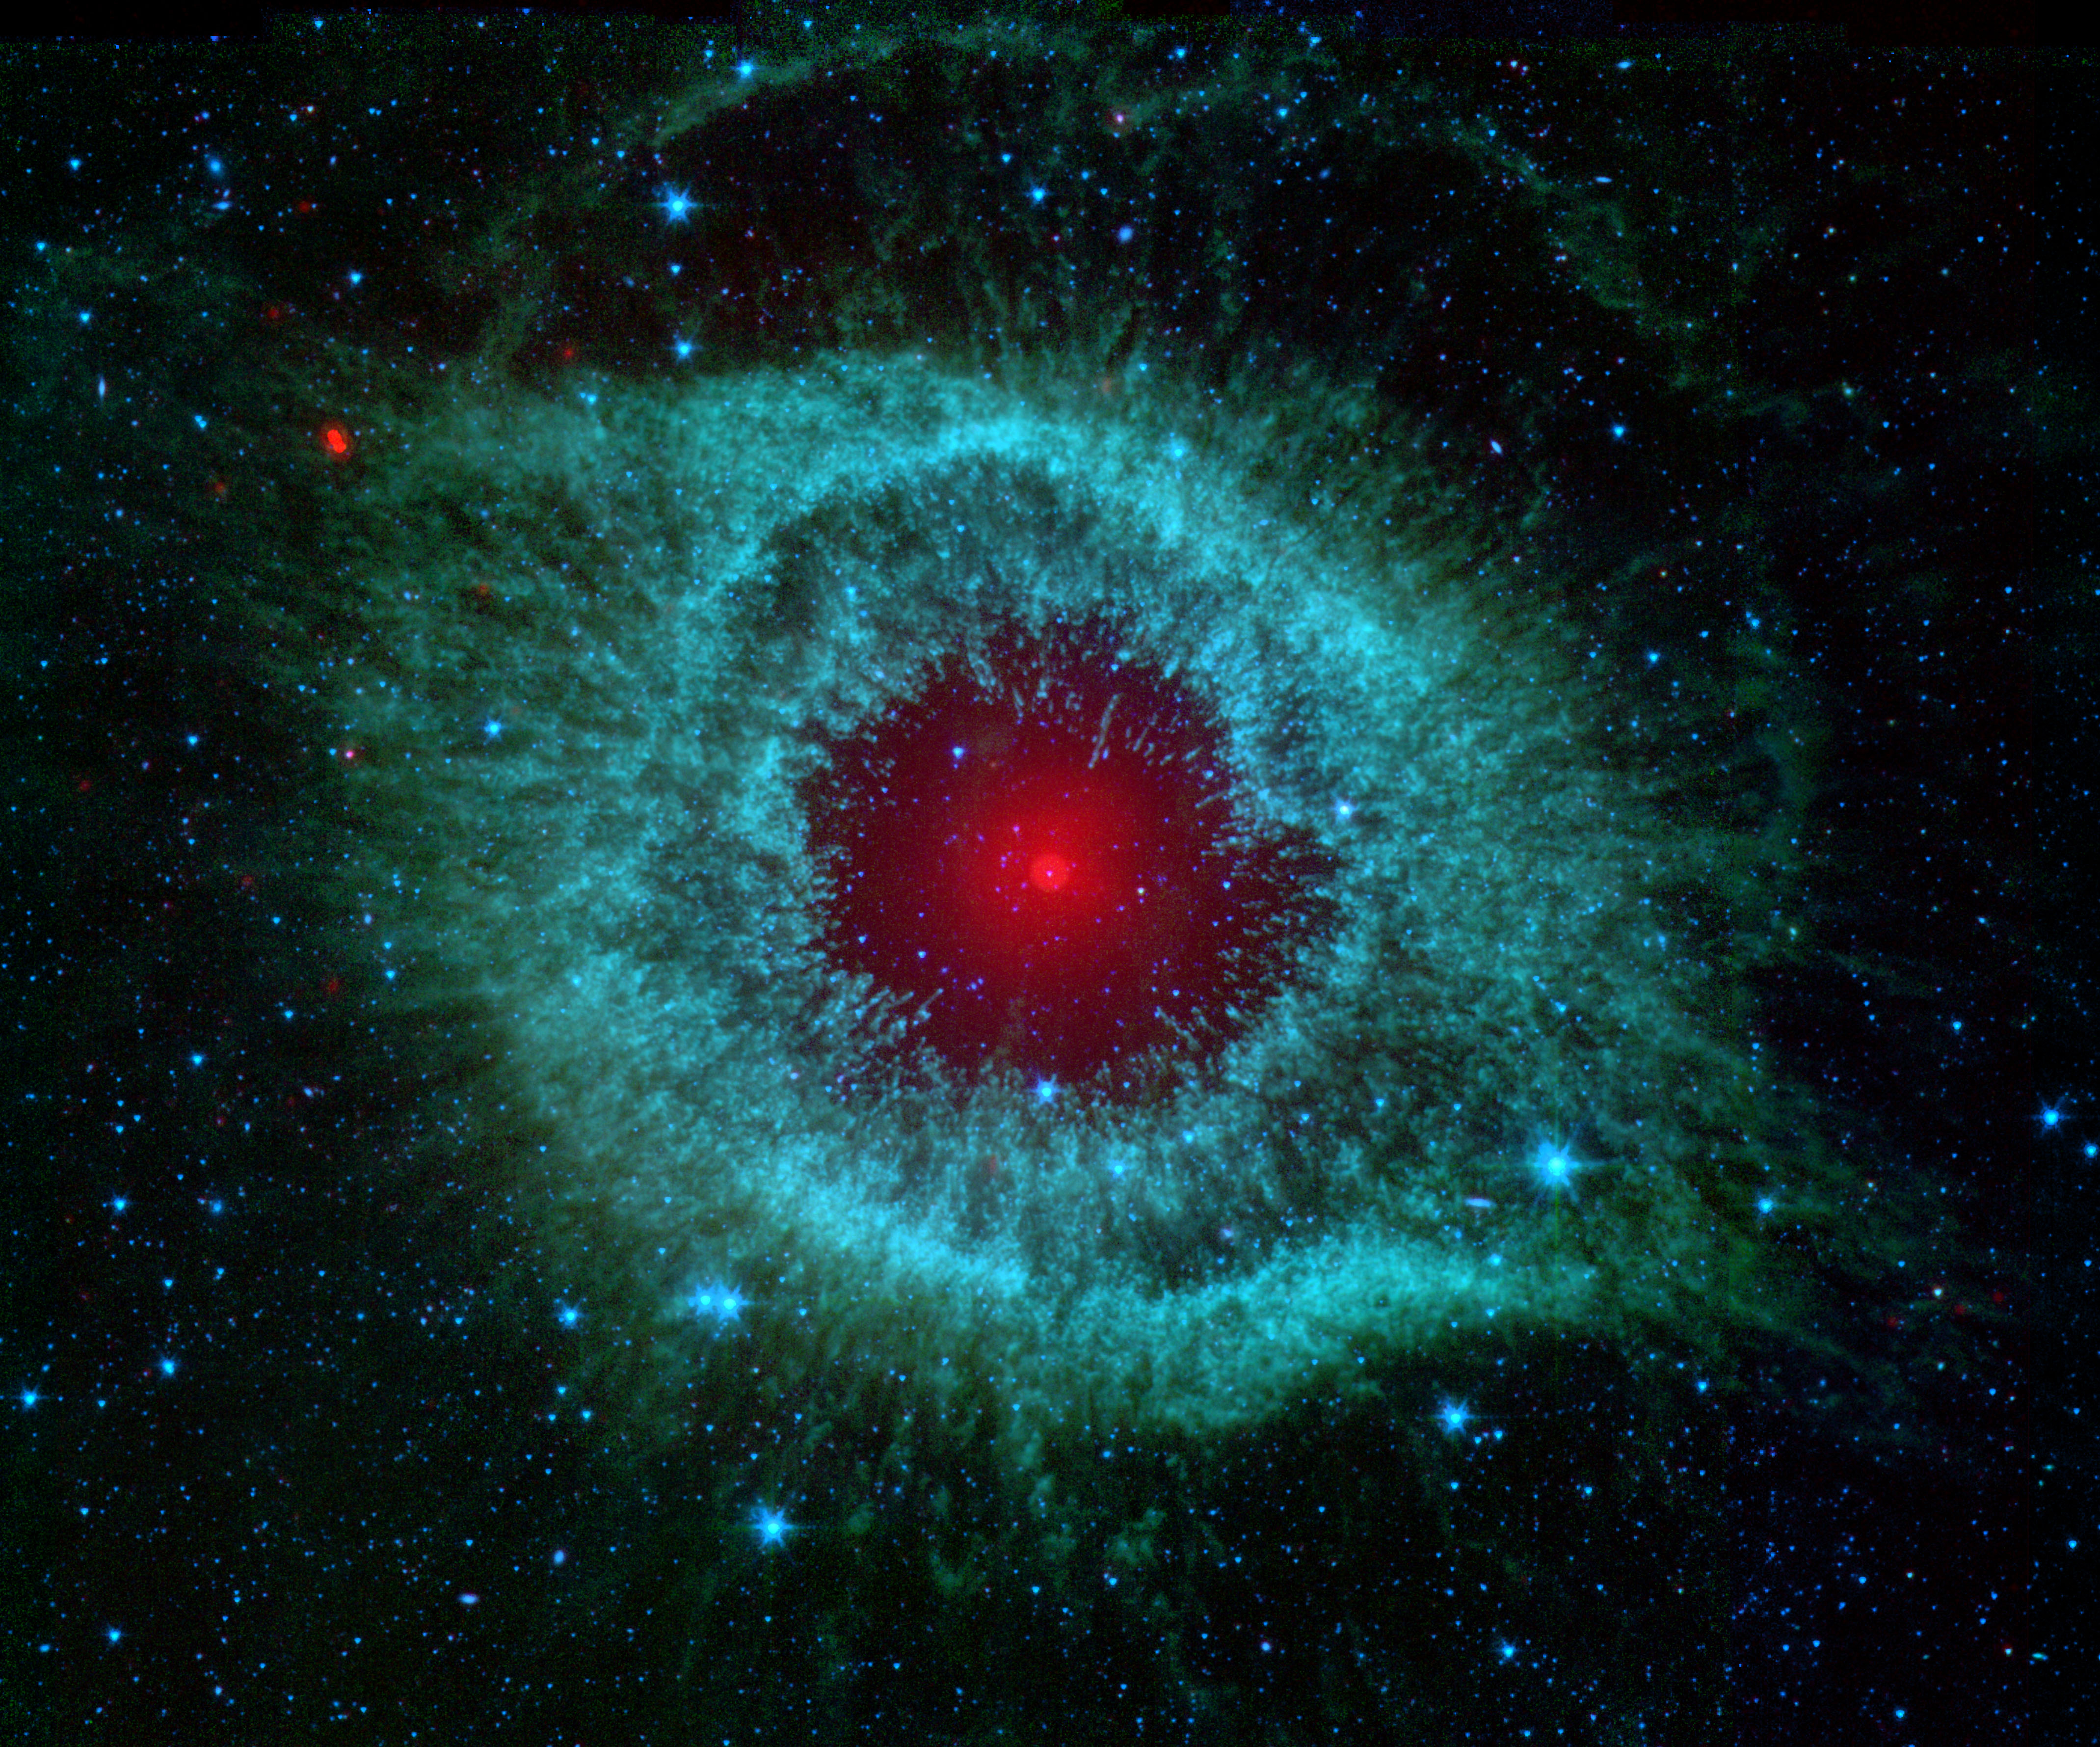
\includegraphics[height=110px]{Helix_Nebula.jpg}
            \vspace*{-5ex}
            \caption{Туманність Равлик в ІЧ спектрі. Пил такої форми утворено саме розкиданими кометами. 2007\cite{7}}
        \end{minipage}
        \hfill
        \begin{minipage}[t]{0.29\textwidth}
            \includegraphics[height=110px]{Hale-Bopp.jpg}
            \vspace*{-2ex}
            \caption{Комета C/1995 O1 (Гейла --- Боппа), одна з найяскравіших за декілька останніх десятиліть. 04.04.1997\cite{8}}
        \end{minipage}
        \vspace*{-2ex}
    \end{figure}
    
    Ці явища зумовлені впливом сонячної радіації та сонячного вітру, що діють на ядро комети. Ядра комети мають діаметри від декількох сотень метрів до десятків кілометрів і складаються з пухкої маси льоду, пилу та дрібних кам'янистих частинок. Кома може бути до 15 разів більше діаметра Землі, тоді як хвіст може розтягуватися на одну астрономічну одиницю. Якщо комета достатньо яскрава, вона може бути помічена із Землі без допомоги телескопа і може стягувати на небі $30\degree$-ну дугу (60 Місяців)\cite{9}. Комети спостерігаються і фіксуються з давніх часів багатьма культурами.

    Комети зазвичай мають еліптичні орбіти з великим ексцентриситетом і широкий діапазон орбітальних періодів, починаючи від декількох років до, потенційно, декількох мільйонів років. Комети короткого періоду зароджуються в поясі Койпера або пов'язаному з ним розсіяному диску\cite{10}, що лежить поза орбітою Нептуна. Вважається, що комети довготривалого періоду беруть початок у хмарі Оорта\cite{11} (Рис.~\ref{Oort}) --- сферичній хмарі льодяних тіл, що починається у зовнішньому поясі Койпера і займає половину відстані до найближчої зірки. Довгоперіодичні комети рухаються до Сонця із хмари Оорта гравітаційними збуреннями (пертурбаціями), що спричиняються приливними силами галактик та зірками, що минають. Гіперболічні комети (з ексцентриситетом $\geq 1$) можуть пройти один раз через внутрішню Сонячну систему, перш ніж потрапити в міжзоряний простір.
    
    \begin{figure}[ht]
        \centering
        \vspace*{-2ex}
        \begin{minipage}[t]{0.336\textwidth}
            \includegraphics[height=167px]{Oort.png}
            \vspace*{-5ex}
            \caption{Художня ілюстрація хмари Оорта та поясу Койпера, розміри тіл завищені для наочності}
            \label{Oort}
        \end{minipage}
        \hfill
        \begin{minipage}[t]{0.307\textwidth}
            \includegraphics[height=167px]{surface.jpg}
            \vspace*{-5ex}
            \caption{67P/Чурюмова --- Герасименко з висоти приблизно 16 км у відтінках сірого. 30.09.2016\cite{12}}
            \label{surface}
        \end{minipage}
        \hfill
        \begin{minipage}[t]{0.27\textwidth}
            \includegraphics[height=167px]{Vesta_color.jpg}
            \vspace*{-5ex}
            \caption{Три ударні кратери астероїда 4 Веста, у дійсних кольорах. 2012\cite{13}}
        \end{minipage}
        \vspace*{-2ex}
    \end{figure}
    
    Комети відрізняються від астероїдів наявністю розширеної, гравітаційно незв'язаної атмосфери, що оточує їхні центральні ядра. Ця атмосфера має частини, що називаються комою (центральна частина, що безпосередньо оточує ядро), і хвостом (лінійна смуга, що складається з пилу або газу, видутого з коми світловим тиском Сонця або витіканням плазми сонячного вітру). Однак згаслі (extinct) комети, які багато разів проходили близько до Сонця, втрачають майже весь свій лід та пил, що випаровуються, і можливо, стають схожими на маленькі астероїди. Вважається, що астероїди мають відмінне від комет походження, утворившись всередині орбіти Юпітера, а не у зовнішній Сонячній системі. Відкриття комет головного поясу та малих планет кентаврів\cite{14} розмило відмінність між астероїдами та кометами. На початку 21 століття були відкриті малі тіла з орбітами, як у довгоперіодичних комет, але характеристиками астероїдів внутрішньої сонячної системи, їх назвали кометами Манкса. Вони все ще класифікуються як комети, наприклад, C/2014 S3 (PANSTARRS). З 2013 по 2017 рік було виявлено 27 комет Манкса.
    
    Станом на липень 2019 існує 6619 відомих комет, кількість яких постійно збільшується в міру їхнього виявлення. Однак це становить лише невелику частку від усієї потенційної популяції комет, оскільки резервуар кометних тіл у зовнішній Сонячній системі (у хмарі Оорта) оцінюється в один трильйон. Приблизно одна комета на рік видна неозброєним оком, хоча багато з них тьмяні й непривабливі. Комети були відвідані космічними апаратами, такими як Rosetta Європейського космічного агентства, який став першим, хто висадив на комету спускний апарат, і NASA Deep Impact, який протаранив поверхню комети 9P/Темпеля (випустив у неї 370-ти кілограмовий модуль зі швидкістю ~10.2 км/с в момент зіткнення) для вивчення її внутрішнього складу.
    
    \textbf{Ядро}
    
    \begin{table}[t]
        \centering
        \caption{Властивості деяких комет}\label{Table1}
        \vspace*{1ex}
        \begin{tabular}{cccc}
            \hline
            Назва                           & Розміри (км)              & Щільність (г/см$^3$)  & Маса (кг)\\
            \hline
             1P/Галлея                      & $15\times8\times8$        & 0,6                   & $3\times 10^{14}$\\
             9P/Темпеля                     & $7,6\times6\times4,9$     & 0,62                  & $7,9\times10^{13}$\\
             19P/Бореллі                    & $8\times4\times4$         & 0,3                   & $2,0\times10^{13}$\\
             81P/Вільда                     & $5,5\times4,0\times3,3$   & 0,6                   & $2,3\times10^{13}$\\
             67P/Чурюмова --- Герасименко   & $4,1\times3,3\times1,8$   & 0,47                  & $1,0\times10^{13}$\\
            \hline 
        \end{tabular}
        \vspace*{-3ex}
    \end{table}
    
    Тверда серцевинна структура комети відома як ядро. Кометні ядра складаються зі суміші каменю, пилу, водного льоду та замерзлого вуглекислого газу, оксиду вуглецю, метану та аміаку. Багато комет мають вищий вміст пилу ніж льоду. Поверхні комет утворені із щільного кристалічного льоду, змішаного з органічними сполуками, тоді як внутрішній лід холодніший і менш щільний.
    
    Поверхня ядра (Рис.~\ref{surface}), як правило, суха, запилена або кам'яниста\cite{15}, це говорить про те, що лід міститься під поверхневою кіркою товщиною кілька метрів. Крім уже згаданих газів, ядра містять різноманітні органічні сполуки, які можуть включати метанол, ціанистий водень, формальдегід, етанол, етан і, можливо, складніші молекули, такі як довголанцюгові вуглеводні та амінокислоти. У 2009 році було підтверджено, що в кометному пилу, вилученому місією NASA Stardust, було виявлено гліцин. У серпні 2011 р. Було опубліковано звіт, оснований на дослідженнях NASA щодо метеоритів, виявлених на Землі, який стверджує, що компоненти ДНК та РНК (аденін, гуанін та споріднені органічні молекули) можуть формуватися на астероїдах та кометах.
    
    Зовнішні поверхні кометних ядер мають дуже низький альбедо. Це робить їх одними з об’єктів Сонячної системи, що найменше відбивають світло. Космічний зонд Giotto виявив, що ядро комети Галлея відбиває близько чотирьох відсотків світла, що падає на нього, а Deep Space 1 виявив, що поверхня комети Бореллі відбиває менш ніж 3,0\%; для порівняння, асфальт відбиває сім відсотків. Матеріал темної поверхні ядра може складатися зі складних органічних сполук. Тепло від Сонця посуває легші леткі сполуки, залишаючи важчі органічні, що, як правило, дуже темні, такі як дьоготь або сира нафта. Темність кометних поверхонь дає їм змогу поглинати тепло, що є рушійною силою їхнього процесу дегазації.
    
    Спостерігалися ядра комети радіусами до 30 кілометрів, але встановити їхній точний розмір важко. Ядро 322P/СОГО, першої періодичної комети, виявленої за допомогою автоматизованих космічних телескопів SOHO, ймовірно, діаметром лише 100--200 метрів. Попри високу чутливість інструментів, було виявлено нестачу малих комет, що призвело до припущень про дійсну відсутність комет діаметром менше ніж 100 метрів. За оцінками, відомі комети мають середню щільність 0,6 г/см$^3$. Через малу масу ядра комети не набувають сферичної форми під власною гравітацією і тому мають неправильну форму.
    
    Приблизно шість відсотків навколоземних астероїдів вважаються вимерлими ядрами комет, у яких вже не проходить процес дегазації, наприклад, 14827 Гіпнос і 3552 Дон Кіхот.
    
    Результати дослідів космічного апарата Rosetta та Philae показують, що ядро 67P/Чурюмова --- Герасименко не має магнітного поля. Це говорить про те, що магнетизм, можливо, не відігравав ролі в ранньому формуванні планетезималей. Крім того, спектрограф Alice на Rosetta визначив, що електрони (в межах 1 км над ядром комети), які з'являються під дією сонячної радіації на водяні молекули (під фотоіонізацією), а не фотони від Сонця, як думалося раніше, відповідають за деградацію молекул води та вуглекислого газу, що виділяються з ядра комети у її кому. Інструменти на спускному апараті Philae виявили щонайменше шістнадцять органічних сполук на поверхні комети, чотири з яких (ацетамід, ацетон, метил ізоціанат і пропіональдегід) вперше були виявлені на кометі.
    
    \begin{figure}[ht]
        \centering
        \vspace*{-2ex}
        \begin{minipage}[t]{0.356\textwidth}
            \includegraphics[height=203px]{SWAN.jpg}
            \vspace*{-2ex}
            \caption{Комета SWAN, що зайшла із зовнішньої Сонячної системи. 2020\cite{16}}
        \end{minipage}
        \hfill
        \begin{minipage}[t]{0.626\textwidth}
            \includegraphics[height=203px]{ATLAS.jpg}
            \vspace*{-5ex}
            \caption{Комета C/2019 Y4 (ATLAS). 2020\cite{17}}
        \end{minipage}
        \vspace*{-2ex}
    \end{figure}
    
    \textbf{Кома}

    Потоки пилу та газу виділяються так, що утворюють навколо комети величезну і надзвичайно тонку атмосферу, яку називають "комою". Сила, що чиниться на кому тиском випромінювання Сонця та сонячним вітром, утворює величезний "хвіст", який спрямовується проти Сонця.
    
    Кома, як правило, складається з води та пилу, водночас вода складає до 90\% летючих речовин, які витікають з ядра, коли комета перебуває в межах від 3 до 4 астрономічних одиниць (450 000 000 до 600 000 000 км) від Сонця. Первинна молекула Н$_2$О руйнується в основному внаслідок фотодисоціації та значно меншою мірою фотоіонізацією, при цьому сонячний вітер відіграє незначну роль у руйнуванні води у порівнянні з фотохімією. Більш великі частинки пилу залишаються вздовж орбітального шляху комети, тоді як дрібні частинки світловим тиском відштовхуються від Сонця у хвіст комети.
    
    Хоча тверде ядро комет, як правило, менше ніж 60 кілометрів у діаметрі, кома може простягатися на тисячі або мільйони кілометрів, а іноді стає більшою за Сонце. Наприклад, приблизно через місяць після спалаху в жовтні 2007 року комета 17P/Голмса ненадовго мала атмосферу пилу більшу, ніж Сонце. У Великої комети 1811 року кома також була приблизно діаметром з Сонце. Попри те, що кома може стати досить великою, її розмір може зменшитися приблизно в той час, коли вона перетне орбіту Марса приблизно в 1,5 астрономічних одиниць (220 000 000 км) від Сонця. На цій відстані сонячний вітер стає достатньо сильним, щоб видути газ і пил з коми, водночас збільшуючи хвіст. Було помічено, що іонні хвости простягаються на астрономічну одиницю (150 мільйонів км) або більше.
    
    І кома, і хвіст освітлені Сонцем і можуть стати видимими, коли комета проходить через внутрішню Сонячну систему, пил безпосередньо відбиває сонячне світло, а гази світяться від іонізації. Більшість комет занадто слабкі, щоб їх було видно без допомоги телескопа, але кілька з них кожного десятиліття стають достатньо яскравими, щоб їх можна було побачити неозброєним оком. Інколи комета може піддатися величезному і раптовому спалаху газу і пилу, під час якого розмір коми сильно збільшується протягом певного періоду часу. Це сталося у 2007 році з кометою Голмса.
    
    У 1996 році було виявлено, що комети випромінюють рентгенівські промені. Це сильно здивувало астрономів, оскільки випромінювання рентгенівських променів зазвичай пов'язане з дуже високотемпературними тілами. Рентгенівські промені породжуються взаємодією комет із сонячним вітром: коли сильно заряджені іони сонячного вітру пролітають через кометарну атмосферу, вони стикаються з атомами та молекулами комети, "викрадаючи" один або кілька електронів з атома. Цей обмін або перенесення електрона на іон сонячного вітру супроводжується переходом іона в стан спокою з випромінюванням рентгенівських променів і фотонів дальньої ультрафіолетової області спектра.
    
    \textbf{Дуговидна ударна хвиля}
    
    Дуговидна ударна хвиля\cite{18}, або головна ударна хвиля\cite{19} утворюється в результаті взаємодії між сонячним вітром і кометарною іоносферою, що створюється іонізацією газів у комі. Коли комета наближається до Сонця, сонячне світло іонізує гази в комі, а зростання швидкості дегазації викликає розширення коми. Коли сонячний вітер проходить через цю іонну кому, з’являється головна ударна хвиля.
    
    Перші спостереження були зроблені в 1980-х і 90-х роках, коли кілька космічних апаратів пролетіли повз комети 21P/Джакобіні --- Ціннера, 1P/Галлея, і 26P/Грігга --- Скеллерупа. Тоді було встановлено, що хвилі у комет ширші та поступовіші, ніж різкі планетарні, що спостерігаються, наприклад, на Землі. Усі ці спостереження були зроблені поблизу перигелію, коли хвиля найбільш розвинена.
    
    Космічний апарат Rosetta спостерігав хвилю комети 67P/Чурюмова --- Герасименко на ранній стадії розвитку, коли дегазація посилювалася під час підльоту комети до Сонця. Цю молоду ударну хвилю було названо хвилею-немовлям (англ. infant bow shock). Хвиля-немовля є асиметричною і, відносно відстані до ядра, ширшою, ніж повністю розвинена.
    
    \textbf{Хвіст}
    
    У зовнішній Сонячній системі комети залишаються замерзлими та неактивними, і їх надзвичайно важко або неможливо виявити із Землі через їхні невеликі розміри. Спостереженнями космічного телескопа Габбла свідчили про статистичні виявлення неактивних ядер комети в поясі Койпера, але ці виявлення ставилися під сумнів. Коли комета наближається до внутрішньої Сонячної системи, сонячне випромінювання змушує летючі речовини всередині комети випаровуватися і витікати з ядра, переносячи пил із собою.
    
    Потоки пилу та газу утворюють окремі хвости, направлені у різні напрямки. Хвіст пилу залишається позаду комети таким чином, що часто утворює вигнутий хвіст, який називається типом II або пильовим хвостом. Водночас іонний хвіст або хвіст типу I, що складається з газів, завжди спрямований безпосередньо від Сонця, слідуючи за лініями магнітного поля, а не орбітальною траєкторією, оскільки сонячний вітер сильніше впливає на газ, ніж на пил. У таких випадках, як, наприклад, коли Земля проходить через орбітальну площину комети, може бути помітний антихвіст, спрямований у зворотному напрямку до іонних та пилових хвостів. Спостереження за антихвостами значно сприяло виявленню сонячного вітру.
    
    Іонний хвіст утворюється в результаті іонізації сонячним ультрафіолетовим випромінюванням частинок у комі. Після того, як частинки іонізуються, вони набувають позитивного електричного заряду, що, своєю чергою, породжує "індуковану магнітосферу" навколо комети. Комета та її індуковане магнітне поле утворюють перешкоду для частинок сонячного вітру. Оскільки відносна орбітальна швидкість комети та сонячного вітру є надзвуковою, ударна хвиля утворюється попереду від сонячної сторони. У цій хвилі великі концентрації кометарних іонів (їх називають "підхопленими іонами", англ. "pick-up ions") збираються і "навантажують" сонячне магнітне поле плазмою так, що лінії поля "огортають" комету, утворюючи іонний хвіст.
    
    Якщо навантаження на іонний хвіст є достатнім, лінії магнітного поля збігаються до тієї точки, де на деякій відстані уздовж іонного хвоста відбувається магнітне перез'єднання (англ. magnetic reconnection). Це призводить до "події від'єднання хвоста" (англ. "tail disconnection event"). Це спостерігалося неодноразово, наприклад, одна помітна подія була зафіксована 20 квітня 2007 року, коли іонний хвіст Комети 2P/Енке був повністю відірваний, поки комета проходила через корональний викид маси. Цю подію спостерігав космічний зонд STEREO.
    
    У 2013 році вчені ESA повідомили, що іоносфера планети Венера здіймається назовні аналогічно іонному хвосту, який спостерігався за таких же умов.
    
    \textbf{Струми}
    
    Нерівномірне нагрівання може спричинити викид новоутворених газів зі слабкого місця на поверхні ядра комети, як із гейзера. Ці потоки газу та пилу можуть змусити ядро крутитися і навіть розщепитися. У 2010 році було виявлено, що сухий лід (замерзлий вуглекислий газ) може живити струмені речовини. Інфрачервоне зображення 103P/Гартлі 2\cite{20} показує такі струмені, які виходять з поверхні комети та несуть із собою частинки пилу в кому.
    
    \textbf{Екзокомети}
    
    Поза Сонячною системою також було виявлено екзокомети, які можуть бути широко поширеними в Чумацькому Шляху. Першу екзокометну систему було виявлено в 1987 році біля дуже молодої (20 мільйонів років) зірки головної послідовності спектрального класу A на ім'я Бета Живописця. Станом на 2013 рік, використовуючи абсорбційну спектроскопію великих хмар газу, що виділяється кометами при проходженні близько до їхньої зірки, було виявлено 11 екзокометних систем. Упродовж десяти років космічний телескоп Kepler відповідав за пошук планет та інших форм поза Сонячною системою. Перші проходження екзокомет були помічені у лютому 2018 року групою, що складалася з професійних астрономів та любителів, у кривих блиску\cite{21}, записаних космічним телескопом Kepler. Після того, як космічний телескоп Kepler завершив свою роботу у жовтні 2018 року, новий телескоп під назвою TESS взяв на себе місію Кеплера. З моменту запуску TESS, використовуючи криві блиску від TESS, астрономи виявили проходження комет навколо Бети Живописця. З того часу, як астрономи почали використовувати TESS, вони навчилися краще розрізняти екзокомети спектроскопічним методом. Нові планети виявляються методом, який розглядає симетричні мінімуми кривих, які з'являються, коли планета затемнює свою батьківську зірку. Однак після подальшої оцінки кривих блиску було виявлено, що представлені несиметричні закономірності мінімумів викликані хвостом комети або сотнями комет.
    
    \textbf{Номенклатура}
    
    За минулі століття правила іменування комет неодноразово змінювали й уточнювали. До початку XX століття більшість комет називалася по року їхнього виявлення, іноді з додатковими уточненнями щодо яскравості або пори року, якщо комет в цьому році було кілька. Наприклад, «Велика комета 1680 року», «Велика вереснева комета 1882 року», «Денна комета 1910 року» («Велика січнева комета 1910 року»).
    
    Після того, як Галлей довів, що комети 1531, 1607 і 1682 років --- це та сама комета, і передбачив її повернення в 1759 році, ця комета стала називатися кометою Галлея. Друга і третя відомі періодичні комети отримали імена Енке і Біели на честь вчених, що обчислили їхні орбіти, попри те, що перша комета спостерігалася ще Мешеном, а друга --- Мессьє у XVIII столітті. Пізніше періодичні комети зазвичай називали на честь їхніх першовідкривачів. Комети, що спостерігалися лише в одному проходженні перигелію, продовжували називати за роком появи.

    На початку XX століття, коли відкриття комет стали частими подіями, було укладено угоду про іменування комет, яка досі залишається актуальною. Комета отримує власне ім'я тільки після того, як її виявлять троє незалежних спостерігачів. В останні роки безліч комет відкривається за допомогою інструментів, які обслуговують великі команди вчених; у таких випадках комети іменуються за інструментом. Наприклад, комета C/1983 H1 (IRAS --- Аракі --- Алкока) була незалежно відкрита супутником IRAS і любителями астрономії Ген'ічі Аракі й Джорджем Алкоком. У минулому, якщо одна група астрономів відкривала кілька комет, до імен додавали номер (але тільки для періодичних комет), наприклад, комети Шумейкерів --- Леві 9. Зараз низкою інструментів щорічно відкривається безліч комет, що зробило таку систему непрактичною. Замість цього використовують спеціальну систему позначення комет.
    
    До 1994 року кометам спочатку давали тимчасові позначення, що складалися з року їхнього відкриття і латинської малої літери, яка вказувала порядок їхнього відкриття в році (наприклад, комета Беннетта була дев'ятою кометою, відкритою в 1969 році, і при відкритті отримала тимчасове позначення 1969i). Після того, як комета проходила перигелій, її орбіта надійно встановлювалася, і комета отримувала постійне позначення, яке складалося з року проходження перигелію і римського числа, що вказувало на порядок проходження перигелію в даному році. Так, комети 1969i було дано постійне позначення 1970 II (друга комета, яка пройшла перигелій в 1970 році).
    
    \textbf{Доля комет}
    \begin{enumerate}
        \item Виліт (викидання) із Сонячної системи 
        
        Якщо комета мандрує достатньо швидко, вона може покинути Сонячну систему. Такі комети рухаються по незамкнених гіперболічних орбітах, і як такі звуться гіперболічними кометами. Нині відомо, що комети викидаються лише при взаємодії з іншим об'єктом Сонячної системи, таким як Юпітер. Прикладом цього вважається комета С/1980 Е1, яка у 1980 році була зміщена з передбаченої орбіти в 7,1 мільйона років навколо Сонця на гіперболічну траєкторію після близького проходу біля Юпітера.
        
        \item Вичерпування летючих речовин 
        
        Комети сімейства Юпітера (КСЮ) та довгоперіодичні комети, як виявилося, слідують дуже різним законам згасання. КСЮ активні протягом життя приблизно 10000 років або ~1000 орбіт, тоді як комети з тривалим періодом обертання зникають набагато швидше. Лише 10\% довгоперіодичних комет існують понад 50 проходів до малого перигелію, і лише 1\% з них переносить понад 2000 проходів. Врешті-решт більша частина летючого матеріалу, що міститься в ядрі комети, випаровується, і комета стає малим темним інертним клаптиком каменю або щебеню, який може нагадувати астероїд. Деякі астероїди на еліптичних орбітах зараз ідентифікуються як вимерлі комети. Приблизно шість відсотків навколоземних астероїдів вважаються вимерлими кометними ядрами.
        
        \item Ламання та зіткнення 
        
        Ядро деяких комет може бути крихким: висновок підкріплений спостереженнями за розщепленням комет. Значним розривом комети був розрив Шумейкерів --- Леві 9, який було виявлено в 1993 році. Близька зустріч у липні 1992 р. розірвала комету на частини, і за шість днів у липні 1994 р. її шматки впали в атмосферу Юпітера --- вперше астрономи спостерігали зіткнення двох об'єктів у Сонячній системі. Іншими кометами, що розпадалися, були 3D/Біели в 1846 р. та 73P/Швассмана --- Вахмана з 1995 по 2006 рр. Грецький історик Ефор повідомляв, що комета розколювалася ще взимку 372--373 рр. до н. е. Передбачається, що розщеплення комет викликаються перепадами температур, тиском внутрішнього газу або зіткненнями.
    \end{enumerate}
    
    \begin{thebibliography}{3}
        % Source
        {\small\bibitem{1} \url{https://solarsystem.nasa.gov/asteroids-comets-and-meteors/comets}}
        {\small\bibitem{2} \href{https://uk.wikipedia.org/wiki/\%D0\%9A\%D0\%BE\%D0\%BC\%D0\%B5\%D1\%82\%D0\%B0}{https://uk.wikipedia.org/wiki/Комета}}
        {\small\bibitem{3} \href{https://ru.wikipedia.org/wiki/\%D0\%9A\%D0\%BE\%D0\%BC\%D0\%B5\%D1\%82\%D0\%B0}{https://ru.wikipedia.org/wiki/Комета}}
        
        % Citations
        {\small\bibitem{4}      \url{https://en.wikipedia.org/wiki/Coma_(cometary)}}
        {\small\bibitem{5}      \url{https://en.wiktionary.org/wiki/comet#Etymology}}
        {\small\bibitem{6}      \url{https://en.wikipedia.org/wiki/Comet_tail}}
        {\small\bibitem{7}      \url{https://www.nasa.gov/mission_pages/spitzer/multimedia/pia09178.html}}
        {\small\bibitem{8}      \url{https://commons.wikimedia.org/wiki/File:Comet_Hale-Bopp_1995O1.jpg}}
        {\small\bibitem{9}      \url{https://en.wikipedia.org/wiki/Subtended_angle}}
        {\small\bibitem{10}     \url{https://en.wikipedia.org/wiki/Scattered_disc}}
        {\small\bibitem{11}     \url{https://en.wikipedia.org/wiki/Oort_cloud}}
        {\small\bibitem{12}     \url{https://solarsystem.nasa.gov/resources/506/comet-from-16-km/?category=small-bodies_comets}}
        {\small\bibitem{13}     \url{https://solarsystem.nasa.gov/resources/1826/near-true-color-image-of-snowman/?category=small-bodies_comets}}
        {\small\bibitem{14}     \url{https://en.wikipedia.org/wiki/Centaur_(small_Solar_System_body)}}
        {\small\bibitem{15}     \url{https://en.wikipedia.org/wiki/67P/Churyumov\%E2\%80\%93Gerasimenko#/media/File:67P_Churyumov-Gerasimenko_surface.gif}}
        {\small\bibitem{16}     \url{https://apod.nasa.gov/apod/ap200429.html}}
        {\small\bibitem{17}     \url{https://apod.nasa.gov/apod/ap200321.html}}
        {\small\bibitem{18}     \url{https://en.wikipedia.org/wiki/Bow_shock}}
        {\small\bibitem{19}     \href{https://ru.wikipedia.org/wiki/\%D0\%93\%D0\%BE\%D0\%BB\%D0\%BE\%D0\%B2\%D0\%BD\%D0\%B0\%D1\%8F_\%D1\%83\%D0\%B4\%D0\%B0\%D1\%80\%D0\%BD\%D0\%B0\%D1\%8F_\%D0\%B2\%D0\%BE\%D0\%BB\%D0\%BD\%D0\%B0}{https://ru.wikipedia.org/wiki/Головная\_ударная\_волна}}
        {\small\bibitem{20}     \url{https://apod.nasa.gov/apod/ap101123.html}}
        {\small\bibitem{21}     \url{https://en.wikipedia.org/wiki/Light_curve}}
        
        % Miscellaneous
        {\small\bibitem{22} \url{https://en.wikipedia.org/wiki/List_of_minor_planets_and_comets_visited_by_spacecraft#List_of_comets_visited_by_spacecraft}}
    \end{thebibliography}

\end{document}